\subsection{Pengujian Gerakan}
\label{subsec:movementtesting}

\begin{figure} [ht]
  \centering
  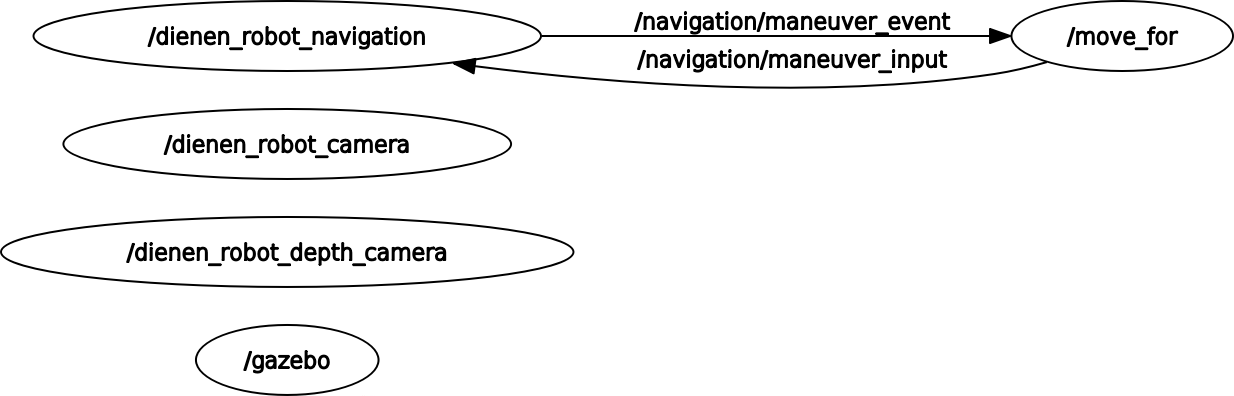
\includegraphics[width=0.45\textwidth]{figures/rosgraph/movement-sim.png}
  \IfLanguageName{english}{
    \caption{Node scheme of the movement testing in the simulation.}
  }{
    \caption{Skema \emph{node} pengujian gerakan di simulasi.}
  }
  \label{fig:rosgraphmovementsim}
\end{figure}

\begin{figure} [ht]
  \centering
  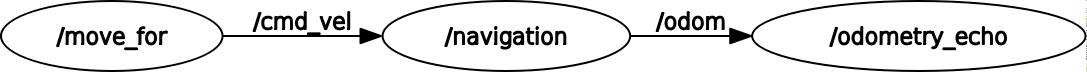
\includegraphics[width=0.45\textwidth]{figures/rosgraph/movement-real.png}
  \IfLanguageName{english}{
    \caption{Node scheme of the movement testing in the real robot.}
  }{
    \caption{Skema \emph{node} pengujian gerakan pada \emph{real robot}.}
  }
  \label{fig:rosgraphmovementreal}
\end{figure}


Pengujian gerakan dilakukan dengan menjalankan \emph{node} \lstinline{move_for} sebagai \emph{node behavior} yang akan memerintahkan robot untuk bergerak dengan kecepatan tertentu selama kurun waktu tertentu.
Seperti yang terlihat pada Gambar \ref{fig:rosgraphmovementsim},
  di simulasi,
  \emph{node} \lstinline{move_for} akan terhubung dengan \emph{node} \lstinline{navigation_plugin} untuk mengatur kecepatan dari robot yang ada di simulasi menggunakan \emph{topic} \lstinline{/navigation/maneuver_input}.
Sedangkan untuk pengujian di dunia nyata, seperti yang terlihat pada Gambar \ref{fig:rosgraphmovementreal},
  peran dari \emph{node} \lstinline{navigation_plugin} yang mengatur navigasi pada robot virtual akan digantikan oleh \emph{node} \lstinline{navigation} yang mengatur navigasi yang ada pada robot fisik.


\begin{figure}[ht]
  \centering
  \begin{tikzpicture}
    \begin{axis}[
        height=0.2\textwidth,
        width=0.45\textwidth,
        ylabel=\IfLanguageName{english}{Distance}{Jarak} (meter),xlabel=\IfLanguageName{english}{$K^{th}$ Attempt}{Percobaan Ke-$K$},
        legend style={
          at={(0.5,1.5)},
          anchor=north,
          legend columns=-1,
        },
        ymajorgrids,
        bar width=3pt,
        ybar=0pt,
        xmin=0.1,
        xmax=12.9,
        ymin=0,
        xtick distance=1,
        ytick distance=1,
      ]
      \addplot table[x=index,y=expecteddistance,col sep=comma]{data/linear-movement-sim.csv};
      \addplot table[x=index,y=measureddistance,col sep=comma]{data/linear-movement-sim.csv};
      \addplot table[x=index,y=odometrydistance,col sep=comma]{data/linear-movement-sim.csv};
      \IfLanguageName{english}{
        \legend{Estimated,Measurement,Odometry}
      }{
        \legend{Perkiraan,Pengukuran,Odometri}
      }
    \end{axis}
  \end{tikzpicture}
  \IfLanguageName{english}{
    \caption{Comparison of last distance results from the expected and measured values in the simulation.}
  }{
    \caption{Perbandingan hasil jarak akhir dari nilai yang diharapkan dan yang terukur di simulasi.}
  }
  \label{fig:linearmovementsim}
\end{figure}


\begin{figure}[ht]
  \centering
  \begin{tikzpicture}
    \begin{axis}[
        height=0.19\textwidth,
        width=0.45\textwidth,
        ylabel=\IfLanguageName{english}{Angle}{Sudut} (degree),xlabel=\IfLanguageName{english}{$K^{th}$ Attempt}{Percobaan Ke-$K$},
        legend style={
          at={(0.5,1.5)},
          anchor=north,
          legend columns=-1,
        },
        ymajorgrids,
        bar width=5pt,
        ybar=0pt,
        xmin=0.1,
        xmax=6.9,
        ymin=0,
        xtick distance=1,
        ytick distance=90,
      ]
      \addplot table[x=index,y=expected,col sep=comma]{data/angular-movement-sim.csv};
      \addplot table[x=index,y=measured,col sep=comma]{data/angular-movement-sim.csv};
      \addplot table[x=index,y=odometry,col sep=comma]{data/angular-movement-sim.csv};
      \IfLanguageName{english}{
        \legend{Estimated,Measurement,Odometry}
      }{
        \legend{Perkiraan,Pengukuran,Odometri}
      }
    \end{axis}
  \end{tikzpicture}
  \IfLanguageName{english}{
    \caption{Last orientation results of angular movement in the simulation.}
  }{
    \caption{Hasil orientasi akhir dari gerakan putar di simulasi.}
  }
  \label{fig:angularmovementsim}
\end{figure}


Pengujian gerakan terbagi menjadi dua bagian,
  pengujian gerakan linier dan pengujian gerakan putar,
  masing-masing diujikan dengan berbagai macam kombinasi nilai kecepatan selama 3 detik pada robot virtual di lingkungan simulasi dan pada robot fisik di dunia nyata.
Seperti yang terlihat pada Gambar \ref{fig:linearmovementsim} dan Gambar \ref{fig:angularmovementsim},
  jarak dan orientasi akhir odometri yang diterima robot memiliki nilai yang relatif sama dengan jarak dan orientasi akhir dari nilai perkiraan dari kecepatan yang diberikan dan pengukuran dari titik awal model robot di simulasi.
Dari hasil tersebut, persentase \emph{error} dari nilai odometri dibandingkan rata-rata nilai perkiraan dan pengukuran di simulasi adalah sebesar 2.6\%.


\begin{figure}[ht]
  \centering
  \begin{tikzpicture}
    \begin{axis}[
        height=0.2\textwidth,
        width=0.45\textwidth,
        ylabel=\IfLanguageName{english}{Distance}{Jarak} (meter),
        xlabel=\IfLanguageName{english}{K Attempt}{Percobaan Ke-},
        legend style={
          at={(0.5,1.5)},
          anchor=north,
          legend columns=-1,
        },
        ymajorgrids,
        bar width=3pt,
        ybar=0pt,
        xmin=0.1,
        xmax=12.9,
        ymin=0,
        xtick distance=1,
        ytick distance=1,
      ]
      \addplot table[x=index,y=expecteddistance,col sep=comma]{data/linear-movement-real.csv};
      \addplot table[x=index,y=measureddistance,col sep=comma]{data/linear-movement-real.csv};
      \addplot table[x=index,y=odometrydistance,col sep=comma]{data/linear-movement-real.csv};
      \IfLanguageName{english}{
        \legend{Expected,Measured,Odometry}
      }{
        \legend{\emph{Expected},\emph{Measured},\emph{Odometry}}
      }
    \end{axis}
  \end{tikzpicture}
  \IfLanguageName{english}{
    \caption{Last distance results of linear movement in the real robot.}
  }{
    \caption{Hasil jarak akhir dari gerakan linier pada \emph{real robot}.}
  }
  \label{fig:linearmovementreal}
\end{figure}


\begin{figure}[ht]
  \centering
  \begin{tikzpicture}
    \begin{axis}[
        height=0.21\textwidth,
        width=0.45\textwidth,
        ylabel=\IfLanguageName{english}{Angle}{Sudut} (degree),
        xlabel=\IfLanguageName{english}{$K^{th}$ Attempt}{Percobaan Ke-$K$},
        legend style={
          at={(0.5,1.5)},
          anchor=north,
          legend columns=-1,
        },
        ymajorgrids,
        bar width=5pt,
        ybar=0pt,
        xmin=0.1,
        xmax=6.9,
        ymin=0,
        xtick distance=1,
        ytick distance=90,
      ]
      \addplot table[x=index,y=expected,col sep=comma]{data/angular-movement-real.csv};
      \addplot table[x=index,y=measured,col sep=comma]{data/angular-movement-real.csv};
      \addplot table[x=index,y=odometry,col sep=comma]{data/angular-movement-real.csv};
      \IfLanguageName{english}{
        \legend{Estimated,Measurement,Odometry}
      }{
        \legend{Perkiraan,Pengukuran,Odometri}
      }
    \end{axis}
  \end{tikzpicture}
  \IfLanguageName{english}{
    \caption{Last orientation results of angular movement on the real robot.}
  }{
    \caption{Hasil orientasi akhir dari gerakan putar pada robot fisik.}
  }
  \label{fig:angularmovementreal}
\end{figure}


Berbeda dengan hasil pengujian di lingkungan simulasi,
  hasil pengujian di dunia nyata memiliki sedikit perbedaan antara nilai perkiraan dan pengukuran dengan nilai odometri yang diterima oleh robot.
Seperti yang terlihat pada Gambar \ref{fig:linearmovementreal} dan Gambar \ref{fig:angularmovementreal},
  terdapat sedikit perbedaan di antara keduanya yang disebabkan oleh kombinasi berbagai faktor seperti ketidakakuratan pembacaan sensor dan terjadinya \emph{slip} ketika robot bergerak dengan akselerasi yang tinggi.
Karena adanya faktor tersebut,
  persentase \emph{error} dari nilai odometri dibandingkan rata-rata nilai perkiraan dan pengukuran pada robot fisik adalah sebesar 12.5\%.
Walaupun begitu,
  terlepas dari adanya perbedaan tingkat akurasi,
  dengan menggunakan \emph{node behavior} yang sama,
  robot tergolong mampu melakukan perintah gerakan yang sesuai ketika diujikan di simulasi maupun di dunia nyata.
